

\section{Motivación e identificación del problema}

\section{Objetivos del trabajo}

\subsection{Objetivo General}

% TODO: refinar
Crear una nueva version del front-end de wikimetrics

\subsection{Objetivos Específicos}

% TUTORIAL: Objetivos mas peque;os que conforman el todo
% También incluye peque;os estudios, decisiones y aprendizajes 

\begin{itemize}{}{}

    \item Implementar una aplicación web responsive que ofrezca las funcionalidades requeridas por un watcher de un wiki y que pueda ser reconocida por los motores de búsqueda.
    \item Consumir y extender la API de wikimetrics para desarrollar una aplicación web que habilite a sus usuarios construir y visualizar gráficas
    \item Definir los requerimientos de la aplicación
    \item Utilizar un método ágil para el desarrollo de la aplicación.
    \item Realizar el despliegue y puesta en producción de la aplicación

\end{itemize}

\section{Estrategia de solución y método de desarrollo ágil a utilizar}
    TODO: DECIDIR ENTRE

    \begin{itemize}
        \item Kanban: Tiene como objetivo la mejora continua, la flexibilidad en la gestión de tareas y un flujo de trabajo mejorado. Con este enfoque ilustrativo, el progreso de todo el proyecto se puede comprender fácilmente de un vistazo. Para esto hace uso del tablero Kanban, que es una herramienta que visualiza todo el proyecto para rastrear el flujo de su proyecto. A través de este enfoque gráfico de los tableros Kanban, un miembro nuevo o una entidad externa puede comprender lo que está sucediendo en este momento, las tareas completadas y las tareas futuras.
        \item Rapid application development (RAD):  es una forma de metodología de desarrollo de software ágil que prioriza las versiones e iteraciones rápidas de prototipos. A diferencia del método Waterfall, RAD enfatiza el uso de software y los comentarios de los usuarios sobre la planificación estricta y el registro de requisitos.
    \end{itemize}

    ELABORAR Y PONER DIBUJITOS ILUSTRATIVOS


\section{Trabajos similares, diferencias y ventajas de la solución a desarrollar}
Siendo wikimedia y wikipedia las mas grandes comunidades y organizaciones dedicadas a recopilar datos, es lógico pensar que tiene consigo una abundante cantidad de seguidores capacitados y apasionados por aportar lo que puedan. A continuación se detallara el estado actual de las herramientas existentes para explorar la wikipedia.

Estas herramientas cumplen diferentes objetivos, 

\begin{enumerate}
    \item Identificar posibles candidatos para ser administrador
    \item Identifica 
    \item Etc.
  \end{enumerate}


\url{https://wikitech.wikimedia.org/wiki/Portal:Toolforge}
\url{https://www.wikidata.org/wiki/Wikidata:Tools/Visualize_data}
\url{https://en.wikipedia.org/wiki/Wikipedia:Tools}

apersonbot.toolforge.org

Este set de herramientas esta enfocado en supervisar usuarios y sus contribuciones a la wikipedia

- Candidate Search
- Aadminscore
- Articles for Creation Review History

\url{https://xtools.wmflabs.org/}


Sin embargo existe una oportunidad para aprovechar mejor la metadata de wikipedia, y explorar y explotar esta sera el problema a resolver de este trabajo especial de grado
\url{https://sigma.toolforge.org/}


\url{https://interaction-timeline.toolforge.org/}


\url{https://cosmiclattes.github.io/wikireplay/player}


\url{https://de.wikipedia.org/wiki/Benutzer:Atlasowa/edit_history_visualization}

\section{Herramientas}

\subsection*{Tecnologías para el ambiente de desarrollo}
\begin{itemize}
    \item Visual Studio Code.
    \item Git, como control de versiones.
    \item Navegadores web (Google Chrome, Firefox, etc)
    \item MongoDB
    \item 
\end{itemize}

\subsection*{Tecnologías o librerías web a utilizar}
\begin{itemize}
    \item Material UI
    \item Next.js + ReactJS
    \item Node
    \item MongoDB
    \item Fastify
\end{itemize}

\section{Requerimientos}
    \begin{enumerate}
        \item{Una herramienta capaz de visualizar graficas sobre propiedades de edicion de un wiki.}
        \item{Los wikis a visualizar son extraídas del watchlist del usuario autenticado a traves de Wikipedia (usando API de MediaWiki).}
        \item{Permitir editar las visualizaciones (alternar tipo de grafica, cambiar los tipos de datos a visualizar).}
        \item{Los datos a representar en las visualizaciones son proporcionados a traves del API Wikimetrics 2.0.}
        \item{La herramienta tiene que ser una aplicacion web.}
        \item{La aplicacion tiene que contar con una vista principal que incluya grafica e informacion general de cada uno de los wiki del watchlist.}
        \item{Permitir al usuario crear una visualizacion nueva y guardarla de forma permanente, para este caso es necesario el uso de una base de datos (preferiblemente MongoDB)}
        \item{La aplicacion tiene que estar alojada en un servidor, para poder ser accedida de manera remota.}
    \end{enumerate}

\section{Prototipo de interfaz}

\subsection{Perfil de Watcher \textbackslash watcher\textbackslash:watcherId}
Para cualquier usuario muestra el perfil de un watcher, en él puedes ver todas las contribuciones de este junto con la lista de visualizaciones que ha creado.
Se permitirá un mínimo de customización. Y se podrá enlazar el perfil de wikipedia


\subsection{Página principal \textbackslash home}
Para usuarios autenticados, les permite ver diferentes secciones relevantes para ellos

\begin{figure}[ht]
    \centering
         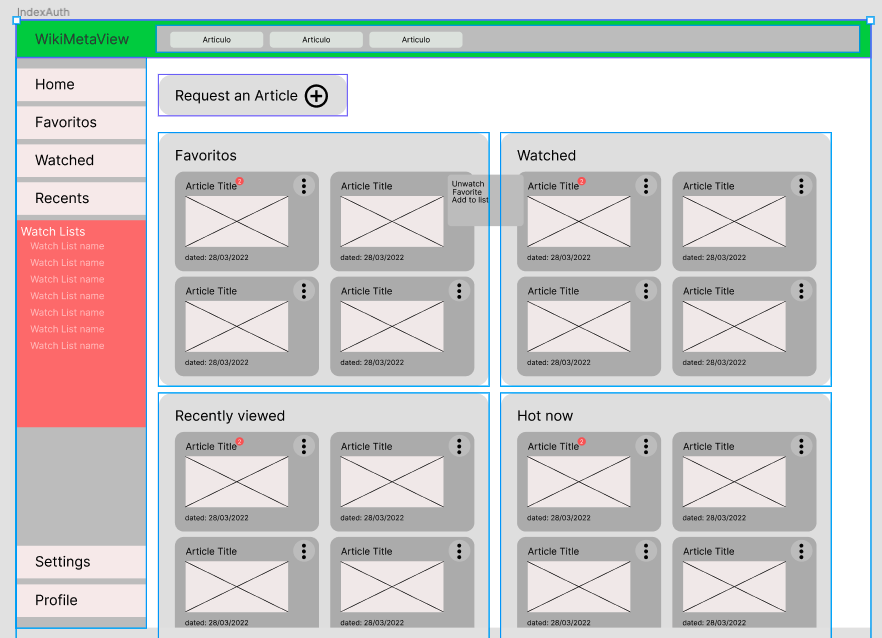
\includegraphics[width=1.0\textwidth]{prototipos/home.png}
          \caption{Normal Case: 1 Request \& 1 Response.}
           \label{normal_case}
\end{figure}


Secciones del home
\begin{enumerate}
    \item Watched \\ Muestra una lista y un pequeño abstracto de los artículos que el usuario hace watching y tienen una visualización actualizada
    \item Queue // Muestra una lista de los artículos que le usuario solicito para hacer una visualización pero que el server no ha podido solicitar
    \item Controversial // Muestra una lista de aquellas visualizaciones que provocan discusión en la comunidad, caracterizado por muchos comentarios
\end{enumerate}


/index
Esta pagina se encarga de explicar las motivaciones de la App y dar una noción básica del funcionamiento para los watchers.
Tiene el objetivo de cap


\subsection{Página de configuración \textbackslash settings}
Acá el usuario puede bla bla 


\subsection{Página de artículo \textbackslash article} 
\url{/article?title=<title>&url=<url>}
Muestra un articulo junto con su metadata y las visualizaciones creadas por los usuarios.d


\subsection{Sobre nosotros \textbackslash about} 
Breve resumen del proyecto, incluye el documento de tesis y documento de seminario asi como datos de contacto y repositorios de github para futuros contribuyentes.

\section{Modales}

Query Params Globales

?auth

Si este parámetro esta en el url. Presenta la modal de autenticación 

?

\section{Planificación de las actividades}

TODO: UNA TABLA DE DOS COLUMNAS

ACTIVIDAD, TIEMPO ESTIMADO.

\begin{lstlisting}
    Preparar el entorno de desarrollo 1/2 semana
    Estudiar API Wikimetrics 2.0 (Back-end) 1/2 semana
    Estudiar API MediaWiki 1/2 semana
    Integracion del API Wikimetrics 2.0 (Back-end) 1/2 semana
    Integracion del API MediaWiki 1/2 semana
\end{lstlisting}